\documentclass[11pt]{article}
\usepackage[margin=1in]{geometry}
\usepackage[utf8]{inputenc}
\usepackage[all]{xy}
\usepackage[hyphens]{url}
\usepackage[hidelinks]{hyperref}

\usepackage{url, hyperref, amsmath, amsfonts, stmaryrd, amssymb, amsthm, mathtools, enumerate, bm, tabularx, graphicx, caption, booktabs, array, ragged2e}
\geometry{letterpaper}
\newtheorem{proposition}{Proposition}

\title{\textbf{Importance Sampling Techniques for Variance Reduction}\\AMS 553: Simulation Modeling and Analysis\\Project Report}
\author{Kai Li\\\href{mailto:kai.li@stonybrook.edu}{\texttt{kai.li@stonybrook.edu}} \and Wenbo Du\\\href{mailto:wenbo.du@stonybrook.edu}{\texttt{wenbo.du@stonybrook.edu}} \and Zhe Zhou\\\href{mailto:zhe.zhou@stonybrook.edu}{\texttt{zhe.zhou@stonybrook.edu}} \and Zeyu Dong\\\href{mailto:zeyu.dong@stonybrook.edu}{\texttt{zeyu.dong@stonybrook.edu}}}
\date{Stony Brook University --- \today}

\begin{document}
\maketitle

\section{Introduction}
Consider the standard Monte Carlo method to find the average value of a function $g(x)$ over an interval $(a, b)$ given by
\[
\frac{1}{b-a} \int_{a}^{b} g(x) dx.
\]
This method generates $m$ replicates $X_{1}, \ldots, X_{m}$ uniformly distributed on $[a, b]$ and estimates the average by the sample mean
\[
\frac{1}{m}\sum_{i=1}^{m} g(X_{i}).
\]
It can be shown that the above quantity converges almost surely to $\frac{1}{b-a}\int_{a}^{b} g(x) dx$ by the strong law of large numbers. However, there are two limitations to this method:
\begin{enumerate}
\item It cannot apply to unbounded intervals.
\item It could be inefficient to draw samples uniformly across the interval if the function $g(x)$ is not very uniform.
\end{enumerate}
It may be more reasonable to consider weight functions or densities besides uniform density, which leads to an effective variance reduction technique called importance sampling. Stratified sampling is found to be effective in reducing variance when a population can be partitioned into subpopulations.

In this report, we will introduce and analyze three different sampling methods: classical importance sampling, stratified sampling, and stratified importance sampling to reduce variance in Monte Carlo simulations. Stratified importance sampling is a combination of importance sampling and stratified sampling. In Sections 2, 3, and 4, we will give some theoretical underpinnings that show the effectiveness in variance reduction of the three methods. We will also analyze the percentage of variance reduction for each method on a given example and compare their performance in simulations in Section 5. The outcome of the simulation matches the theoretical background behind the three methods. That is, we find the three methods succeed in reducing variance.

\section{Importance Sampling}
Suppose $X$ is a random variable with density $f(x)$ supported on $A$, then
\[
\int_A g(x) dx = \int_A \frac{g(x)}{f(x)} f(x) dx = \mathbb{E}_f\left[\frac{g(X)}{f(X)}\right].
\]
We can estimate $\mathbb{E}_f[g(X)/f(X)]$ by simple Monte Carlo integration. In other words, we compute the average
\[
\frac{1}{m} \sum_{i=1}^{m} \frac{g\left(X_{i}\right)}{f\left(X_{i}\right)},
\]
where the random variables $X_{1}, \ldots, X_{m}$ are i.i.d. generated from $f(x)$. The density function $f(x)$ is called the importance function.

The distribution of $X$ can be chosen to reduce the variance of the sample mean estimator. It can be shown that the minimum variance is obtained when
\[
f(x)=\frac{|g(x)|}{\int_{A}|g(x)| dx}.
\]
This result shows that when choosing the distribution $f(x)$, we want to make sure the value of $g(x)/f(x)$ is close to a constant, or intuitively, we want $f(x)$ to have a similar ``shape'' as $g(x)$. In the meanwhile, though, the variable with density $f(x)$ should be reasonably easy to simulate.

\section{Stratified Sampling}
Stratified sampling is another approach used to reduce variance in simulation studies. The objective is to reduce the variance of the estimator by dividing the interval into strata and estimating the integral on each stratum with a smaller variance. Linearity of the integral operator and the strong law of large numbers imply that the sum of these estimates converges to $\int g(x) d x$ almost surely. In stratified sampling, the number of replicates $m$ and number of replicates $m_{j}$ to be drawn from each of $k$ strata are fixed so that $m=m_{1}+\cdots+m_{k}$, with the goal that
\[
\operatorname{Var}\left(\widehat{\theta}_{k}\left(m_{1}, \ldots, m_{k}\right)\right)<\operatorname{Var}\left(\widehat{\theta}\right),
\]
where $\widehat{\theta}_{k}\left(m_{1}, \ldots, m_{k}\right)$ is the stratified estimator and $\widehat{\theta}$ is the simple Monte Carlo estimator based on $m=m_{1}+\cdots+m_{k}$ replicates.

\begin{proposition}
Let $\widehat{\theta}^{M}$ be the Monte Carlo estimator with $M$ replicates, and let
\[
\widehat{\theta}^{S}=\frac{1}{k} \sum_{j=1}^{k} \widehat{\theta}_{j}
\]
be the stratified estimator with equal size $m=M / k$ strata. Denote the mean and variance of $g(U)$ on stratum $j$ by $\theta_{j}$ and $\sigma_{j}^{2}$, respectively. Then $\operatorname{Var}\left(\widehat{\theta}^{M}\right) \geq \operatorname{Var}\left(\widehat{\theta}^{S}\right)$.
\end{proposition}
\begin{proof}
By independence of $\widehat{\theta}_{j}{ }^{\prime} s$,
\[
\operatorname{Var}\left(\widehat{\theta}^{S}\right)=\operatorname{Var}\left(\frac{1}{k} \sum_{j=1}^{k} \widehat{\theta}_{j}\right)=\frac{1}{k^{2}} \sum_{j=1}^{k} \frac{\sigma_{j}^{2}}{m}=\frac{1}{M k} \sum_{j=1}^{k} \sigma_{j}^{2}.
\]
Now, if $J$ is the randomly selected stratum, it is selected with uniform probability $1 / k$, and applying the conditional variance formula
\begin{align*}
\operatorname{Var}\left(\widehat{\theta}^{M}\right) &=\frac{\operatorname{Var}(g(U))}{M}=\frac{1}{M}(\operatorname{Var}(\mathbb{E}[g(U \mid J)])+\mathbb{E}[\operatorname{Var}(g(U \mid J))])\\
&=\frac{1}{M}\left(\operatorname{Var}\left(\theta_{J}\right)+\mathbb{E}\left[\sigma_{J}^{2}\right]\right) \\
&=\frac{1}{M}\left(\operatorname{Var}\left(\theta_{J}\right)+\frac{1}{k} \sum_{j=1}^{k} \sigma_{j}^{2}\right) \\
&=\frac{1}{M} \operatorname{Var}\left(\theta_{J}\right)+\operatorname{Var}\left(\widehat{\theta}^{S}\right) \geq \operatorname{Var}\left(\widehat{\theta}^{S}\right).
\end{align*}
The inequality is strict except in the case where all the strata have identical means.
\end{proof}
Based on the proof of the proposition, there can be more reduction in variance using stratification when the means of the strata are widely dispersed than if the means of the strata are approximately equal. For integrands that are monotone functions, stratification should be an effective way to reduce variance.

\section{Stratified Importance Sampling}
Stratified importance sampling is a modification to the importance sampling method of estimating $\theta = \int g(x)dx$. Especially, stratified sampling considers sampling from a population that can be partitioned into $k$ subpopulations using the importance function $f(x)=1$.

Similar to the importance sampling method, first we choose a suitable importance function $f$. Suppose that $X$ is generated with density $f$ and c.d.f. $F$ using the probability integral transformation. If $M$ replicates are generated, the importance sampling estimate $\theta$ has variance $\sigma^2/M$, where $\sigma^2=\operatorname{Var}\left(g(X)/f(X)\right)$.

For the stratified importance sampling estimate, divide the real line into $k$ intervals $I_j=\{x:a_{j-1}\leq x <a_j\}$ with endpoints $a_0=-\infty$, $a_j=F^{-1}(j/k)$, where $j=1,\ldots,k-1$, and $a_k=\infty$. On each subinterval define $g_j(x)=g(x)$ if $x\in I_j$ and $g_j(x)=0$ otherwise. Now, we have $k$ parameters to estimate,
\[
\theta_j=\int_{a_{j-1}}^{a_j} g_j(x)dx,\quad j=1,\ldots,k
\]
and $\theta=\theta_1+\cdots+\theta_k$. The conditional densities provide the importance functions on each subinterval. That is, on each subinterval $I_j$, the conditional density $f_j$ of $X$ is defined by
\begin{align*}
f_j(x)=f_{X|I_j}(x|I_j) &=\frac{f(x,a_{j-1}\leq x<a_j)}{\mathbb{P}(a_{j-1}\leq x<a_j)}\\
&=\frac{f(x)}{1/k}=kf(x),\quad a_{j-1}\leq x<a_j.
\end{align*}

Let $\sigma_j^2=\operatorname{Var}\left(g_j(X)/f_j(X)\right)$. For each $j= 1,\ldots,k$ we simulate an importance sample size $m$, compute the importance sampling estimator $\widehat{\theta}_{j}$ of $\theta_j$ on the $j$th subinterval, and compute $\widehat{\theta}^{SI}=\frac{1}{k}\sum_{j=1}^k\widehat{\theta}_{j}$. Then by independence of $\widehat{\theta}_{1},\ldots,\widehat{\theta}_{k}$,
\[
\operatorname{Var}\left(\widehat{\theta}^{SI}\right)=\operatorname{Var}\left(\sum_{j=1}^k\widehat{\theta}_{j}\right)=\sum_{j=1}^k\frac{\sigma_j^2}{m}=\frac{1}{m}\sum_{j=1}^k\sigma_j^2.
\]

Denote the importance sampling estimator by $\widehat{\theta}^{I}$. We can conclude whether $\widehat{\theta}^{SI}$ is better estimator of $\theta$ than $\widehat{\theta}^{I}$ by checking that whether $\operatorname{Var}\left(\widehat{\theta}^{SI}\right)$ is smaller than the variance without stratification. The variance is reduced by stratification if 
\[
\frac{\sigma^2}{M}>\frac{1}{m}\sum_{j=1}^k\sigma_j^2=\frac{k}{M}\sum_{j=1}^k\sigma_j^2 \implies \sigma^2-k\sum_{j=1}^k\sigma_j^2>0.
\]

\begin{proposition}
Suppose $M = mk$ is the number of replicates for an importance sampling estimator $\widehat{\theta}^{I}$, and $\widehat{\theta}^{SI}$ is a stratified importance sampling estimator, with estimates $\widehat{\theta}_{j}$ for $\theta_j$ on the individual strata, each with $m$ replicates. If $\operatorname{Var}\left(\widehat{\theta}^{I}\right)=\sigma^2/M$ and $\operatorname{Var}\left(\widehat{\theta}_{j}\right)=\sigma_j^2/m, j=1,\ldots,k$, then
\[
\sigma^2-k\sum_{j=1}^k \sigma_j^2\geq 0
\]
with equality if and only if $\theta_1=\dots=\theta_k$. Hence, stratification never increases the variance, and there exists a stratification that reduces the variance except when $g(x)$ is constant.
\end{proposition}
\begin{proof}
To determine when the above inequality holds, we need to consider the relation between the random variables with densities $f_j$ and the random variable $X$ with density $f$.

Consider a two-stage experiment. First a number $J$ is drawn at random from the integers 1 to $k$. After observing $J=j$, a random variable $X^*$ is generated from the density $f_j$ and
\[
Y^*=\frac{g_j(x)}{f_j(x)}=\frac{g_j(X^*)}{kf(X^*)}.
\]
To compute the variance of $Y^*$ we apply the conditional variance formula \[
\operatorname{Var}(Y^*)=\mathbb{E}[\operatorname{Var}(Y^*|J)]+\operatorname{Var}(\mathbb{E}[Y^*|J]),
\]
where
\[
\mathbb{E}[\operatorname{Var}(Y^*|J)]=\sum_{j=1}^k\sigma_j^2P(J=j)=\frac{1}{k}\sum_{j=1}^k\sigma_j^2
\]
and $\operatorname{Var}(\mathbb{E}[Y^*|J])=\operatorname{Var}(\theta_J).$ So here we have,
\[
\operatorname{Var}(Y^*)=\frac{1}{k}\sum_{j=1}^k\theta_j^2+\operatorname{Var}(\theta_J).
\]
On the other hand, 
\[
k^2\operatorname{Var}(Y^*)=k^2\mathbb{E}[\operatorname{Var}(Y^*|J)]+k^2\operatorname{Var}(\mathbb{E}[Y^*|J])
\]
and 
\[
\sigma^2=\operatorname{Var}(Y)=\operatorname{Var}(kY^*)=k^2\operatorname{Var}(Y^*)
\]
which imply that
\[
\sigma^2=k^2\operatorname{Var}(Y^*)=k^2\left(\frac{1}{k}\sum_{j=1}^k\sigma_j^2+\operatorname{Var}(\theta_J)\right)=k\sum_{j=1}^k\sigma_j^2+k^2\operatorname{Var}(\theta_J).
\]
Therefore,
\[
\sigma^2-k\sum_{j=1}^k\sigma_j^2=k^2\operatorname{Var}(\theta_J)\geq0,
\]
and equality holds if and only if $\theta_1=\cdots=\theta_k$.
\end{proof}

\section{Simulation Modeling and Analysis}
In this section, we will use the three methods we discussed to estimate
\[
\int_0^1 \frac{e^{-x}}{1+x^2}dx.
\]

\subsection{Importance Sampling}
We have five possible choices of importance functions:
\begin{gather*}
f_0(x)=1,\, 0<x<1,\\
f_1(x)=e^{-x},\, 0<x<\infty,\\
f_2(x)=(1+x^2)^{-1}/\pi,\, -\infty<x<\infty,\\
f_3(x)=e^{-x}/(1-e^{-1}),\, 0<x<1,\\
f_4(x)=4(1+x^2)^{-2}/\pi,\, 0<x<1.
\end{gather*}
In this example, we have
\[
g(x)=
\begin{cases}
e^{-x}/(1+x^2), & \text{if } 0<x<1;\\
0, & \text{otherwise}.
\end{cases}
\]
Notice that the given five importance functions are positive on the support set $0<x<1$ of $g$. However, the support sets of $f_1$ and $f_2$ extend to infinity and a lot of the simulated values will contribute zeros to the sum, which is not efficient. On the other hand, the five distributions are easy to simulate: $f_1$ is exponential distribution with rate 1; $f_2$ is standard Cauchy distribution or $t$ distribution with 1 d.f.; $f_3$ and $f_4$ can be simulated by the inverse transform method.

Fix the number of replicates to 10,000. The densities are plotted on (0, 1) for comparison with $g(x)$ in Figure \ref{fig:1}. The importance function that corresponds to the most nearly constant ratio $g(x)/f(x)$ appears to be $f_3$, which can be seen more clearly in Figure \ref{fig:2}. From the graphs, we might prefer $f_3$ for the smallest variance.

\begin{figure}[h!]
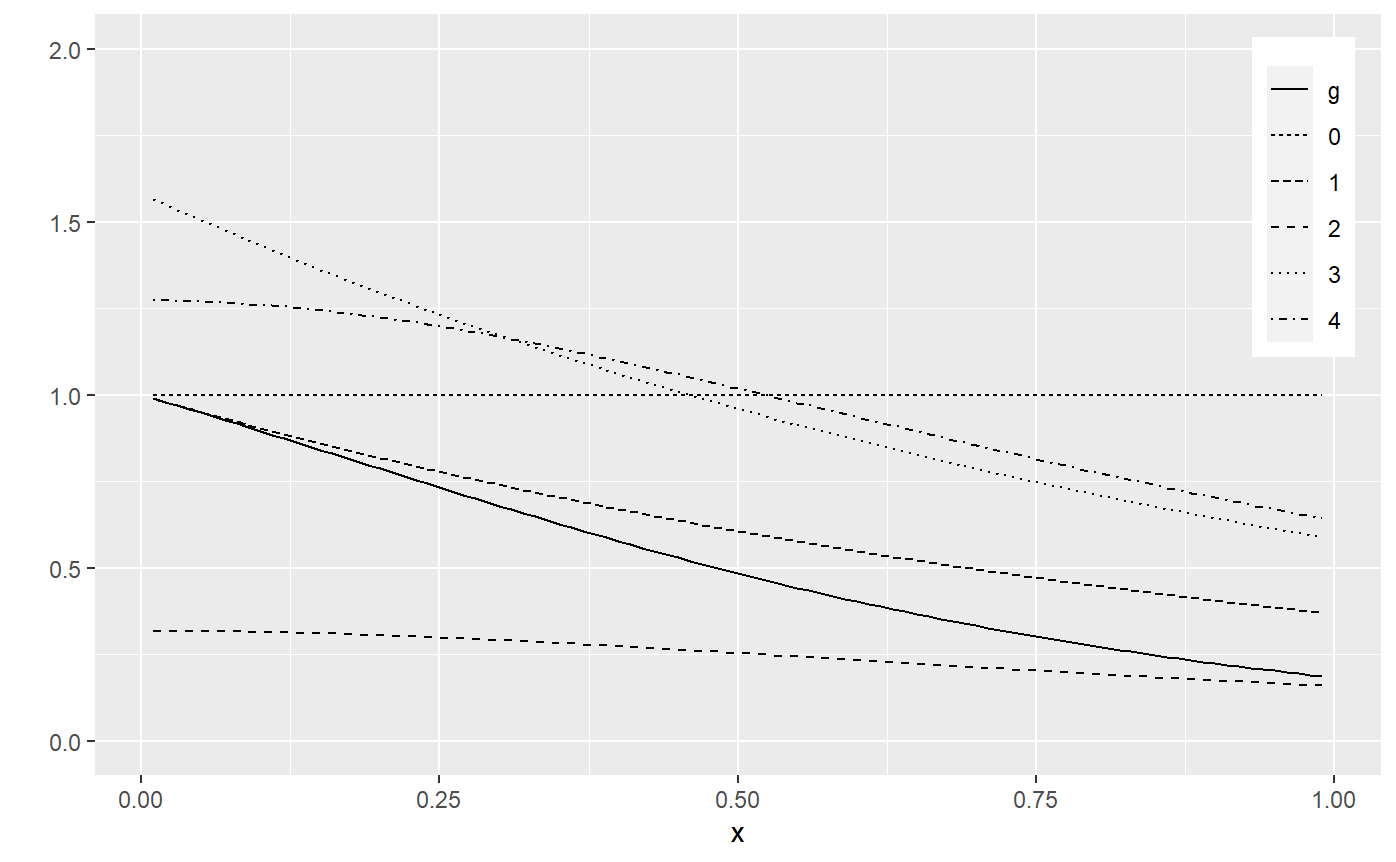
\includegraphics[width=0.95\textwidth]{1}
\centering
\caption{Importance functions $f_0$, $f_1$, $f_2$, $f_3$, $f_4$ (lines 0:4) with $g(x)$}\label{fig:1}
\end{figure}

\begin{figure}[h!]
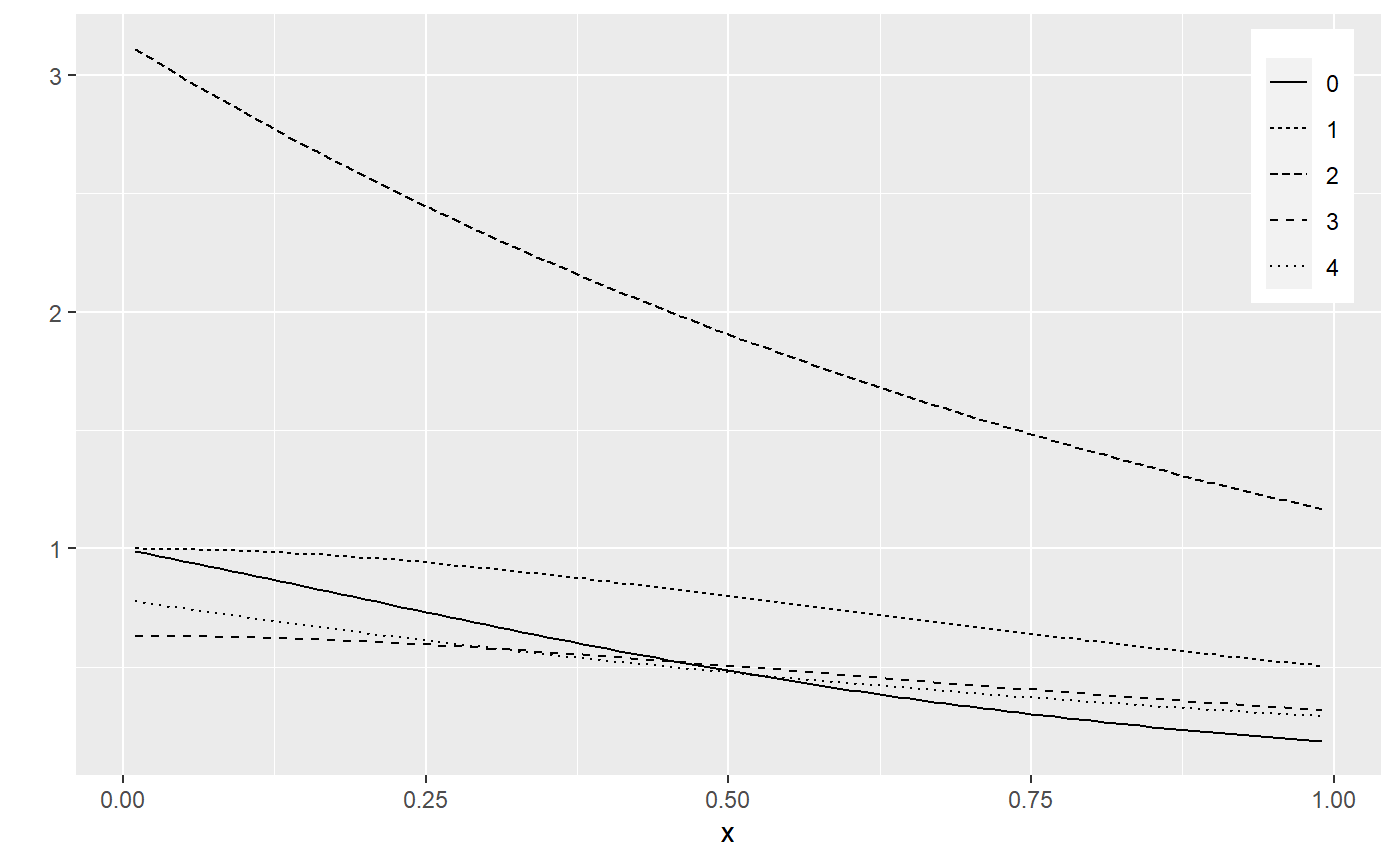
\includegraphics[width=0.95\textwidth]{2}
\centering
\caption{Importance functions $f_0$, $f_1$, $f_2$, $f_3$, $f_4$ (lines 0:4) with $g(x)/f(x)$}\label{fig:2}
\end{figure}

The estimates $\widehat{\theta}^I$ of $\int_0^1e^{-x}(1+x^2)^{-1}dx$ and the corresponding variances are shown in Table \ref{tab:1}. Note that the simulation indicates that $f_3$ and potentially $f_4$ produce the smallest variance among the given five importance functions, while $f_2$ produces the highest variance. An interesting observation is that the standard Monte Carlo estimate without importance sampling has $\operatorname{Var}\left(\widehat{\theta}^I\right)=0.0601$ ($f_0=1$), but $f_1$ and $f_2$ produce higher variances. This implies that the importance functions $f_1$ and $f_2$ do not reduce variance, but $f_3$ and $f_4$ each reduce the variance in estimating $\theta$.

More precisely, simulation using $f_3$ and $f_4$ results in a more than 84\% and 66\% reduction in variance, respectively. This simulation analysis result matches our expectation that the importance function chosen should be an $f$ that is supported on exactly the set where $g(x)>0$, and such that the ratio $g(x)/f(x)$ is nearly constant.

\begin{table}[h!]
\centering
\caption{Estimates and their variances of the integral using importance sampling}\label{tab:1}
\begin{tabular}{ccccccc}
\toprule
$f$ & $f_0$ & $f_1$ & $f_2$ & $f_3$ & $f_4$\\
\midrule
$\widehat{\theta}^I$ & 0.5263 & 0.5238 & 0.5122 & 0.5240 & 0.5233\\
$\operatorname{Var}\left(\widehat{\theta}^I\right)$ & 0.0601 & 0.1750 & 0.9222 & 0.0094 & 0.0202\\
\bottomrule
\end{tabular}
\end{table}

\subsection{Stratified Sampling}
Fix the total number of replicates to 10,000. Also, we fix the number of times to repeat the estimation $N$ to 50. We divide the interval into $k$ subintervals, and compute a Monte Carlo estimate of the integral on each subinterval using $1/k$ of the total number of replicates. Then combine these $k$ estimates to obtain the estimate of $\int_0^1e^{-x}(1+x^2)^{-1}dx$ and compare the variance of the stratified sampling estimator with the standard Monte Carlo estimator. The results are shown in Table \ref{tab:2}.

\begin{table}[h!]
\centering
\caption{Estimates and their variances of the integral using stratified importance sampling}\label{tab:2}
\begin{tabular}{cccccc}
\toprule
$k$ & 1 & 4 & 10 & 50\\
\midrule
$\widehat{\theta}^S$ & 0.5256 & 0.5289 & 0.5248 & 0.5233\\
$\operatorname{Var}\left(\widehat{\theta}^S\right)$ & $5.64\times10^{-6}$ & $3.28\times10^{-7}$ & $4.62\times10^{-8}$ & $2.92\times10^{-9}$\\
\bottomrule
\end{tabular}
\end{table}

Note that $k=1$ represents the standard Monte Carlo method. Simulation using $k=4, 10, 50$ strata results in a more than 94\%, 99\%, and 99\% reduction in variance, respectively, compared to the Monte Carlo method.

\subsection{Stratified Importance Sampling}
Recall that our best result in estimating $\theta$ using the importance sampling method was obtained with importance function $f_3=e^{-x}/(1-e^{-1})$, $0<x<1$. Now divide the interval (0, 1) into $k$ subintervals, $(j/k, (j+1)/k)$, $j=0, 1, \ldots, k-1$. Then on the $j$th subinterval variables are generated from the density
\[
f_j(x)=f_{X|I_j}(x|I_j)=\frac{ke^{-x}}{1-e^{-1}}, \quad\frac{j-1}{k}<x<\frac{j}{k}.
\]

Again, fix the total number of replicates to 10,000. The simulation results for various numbers of subintervals with importance function $f_3$ are shown in Table \ref{tab:3}.

\begin{table}[h!]
\centering
\caption{Estimates and their variances of the integral using stratified sampling}\label{tab:3}
\begin{tabular}{cccccc}
\toprule
$k$ & 1 & 5 & 10 & 20\\
\midrule
$\widehat{\theta}^{SI}$ & 0.5253 & 0.5252 & 0.5250 & 0.5248\\
$\operatorname{Var}\left(\widehat{\theta}^{SI}\right)$ & 0.0093 & $1.73\times10^{-5}$ & $1.09\times10^{-6}$ & $6.95\times10^{-8}$\\
\bottomrule
\end{tabular}
\end{table}

Note that $k=1$ represents the importance sampling method considering $f_3$ to be the importance function. Simulation using $k=5, 10, 20$ strata all results in a more than 99\% reduction in variance compared to the standard importance sampling technique.
\end{document}